\documentclass[letterpaper,11pt,oneside,reqno]{article}

%%%%%%%%%%%%%%%%%%%%%%%%%%%%%%%%%%%%%%%%%%%%%%%%%%%%%%%%%%%%

\usepackage[pdftex,backref=page,colorlinks=true,linkcolor=blue,citecolor=red]{hyperref}
\usepackage[alphabetic,nobysame]{amsrefs}

%%%%%%%%%%%%%%%%%%%%%%%%%%%%%%%%%%%%%%%%%%%%%%%%%%%%%%%%%%%%
%main packages
\usepackage{amsmath,amssymb,amsthm,amsfonts,mathtools}
\usepackage{graphicx,color}
\usepackage{upgreek}
\usepackage[mathscr]{euscript}

%equations
\allowdisplaybreaks
\numberwithin{equation}{section}

%tikz
\usepackage{tikz}
\usetikzlibrary{shapes,arrows,positioning,decorations.markings}

%conveniences
\usepackage{array}
\usepackage{adjustbox}
\usepackage{cleveref}
\usepackage{enumerate}
\usepackage{datetime}
\usepackage{comment}

%paper geometry
\usepackage[DIV=12]{typearea}

%%%%%%%%%%%%%%%%%%%%%%%%%%%%%%%%%%%%%%%%%%%%%%%%%%%%%%%%%%%%
%draft-specific
\synctex=1
% \usepackage{refcheck,comment}

%%%%%%%%%%%%%%%%%%%%%%%%%%%%%%%%%%%%%%%%%%%%%%%%%%%%%%%%%%%%
%this paper specific
\newcommand{\ssp}{\hspace{1pt}}

%%%%%%%%%%%%%%%%%%%%%%%%%%%%%%%%%%%%%%%%%%%%%%%%%%%%%%%%%%%%
\newtheorem{proposition}{Proposition}[section]
\newtheorem{lemma}[proposition]{Lemma}
\newtheorem{corollary}[proposition]{Corollary}
\newtheorem{theorem}[proposition]{Theorem}
%%%%%%%%%%%%%%%%%%%%%%%%%%%%%%%%%%%%%%%%%%%%%%%%%%%%%%%%%%%%
\theoremstyle{definition}
\newtheorem{definition}[proposition]{Definition}
\newtheorem{remark}[proposition]{Remark}
\newtheorem{example}[proposition]{Example}
%%%%%%%%%%%%%%%%%%%%%%%%%%%%%%%%%%%%%%%%%%%%%%%%%%%%%%%%%%%%


\newenvironment{lnotes}{\section*{Notes for the lecturer}}{}
\excludecomment{lnotes}


\begin{document}
\title{Lectures on Random Matrices
(Spring 2025)
\\Lecture 4: Semicircle law for G$\beta$E via tridiagonalization. Beginning determiantal processes}


\date{Wednesday, January 29, 2025\footnote{\href{https://lpetrov.cc/rmt25/}{\texttt{Course webpage}}
$\bullet$ \href{https://lpetrov.cc/simulations/model/random-matrices/}{\texttt{Live simulations}}
$\bullet$ \href{https://lpetrov.cc/rmt25/rmt25-notes/rmt2025-l04.tex}{\texttt{TeX Source}}
$\bullet$
Updated at \currenttime, \today}}



\author{Leonid Petrov}


\maketitle
\tableofcontents

\section{Recap}

Note: I did some live random matrix simulations
\href{https://lpetrov.cc/simulations/2025-01-28-goe/}{here}
and
\href{https://lpetrov.cc/simulations/2025-01-28-bbp-transition/}{here}
--- check them out. More simulations to come.

\subsection{Gaussian ensembles}

We introduced Gaussian ensembles,
and for GOE ($\beta=1$) we computed the joint eigenvalue density.
The normalization is so that the off-diagonal elements have variance $\frac{1}{2}$
and the diagonal elements have variance $1$.
Then the joint eigenvalue density is
\begin{equation*}
	p(\lambda_1,\ldots,\lambda_n)
	=
	\frac{1}{Z_n}\,
	\prod_{i=1}^n e^{-\frac{1}{2}\lambda_i^2}
	\prod_{1\le i<j\le n}(\lambda_i - \lambda_j),
	\qquad
	\lambda_1\ge \lambda_2\ge \ldots \ge \lambda_n.
\end{equation*}

\subsection{Tridiagonalization}

We showed that any real symmetric matrix \(A\) can be tridiagonalized by an orthogonal transformation \(Q\):
\[
	Q^\top\,A\,Q \;=\; T,
\]
where \(T\) is real symmetric tridiagonal, having nonzero entries only on the main diagonal and the first super-/subdiagonals:
\begin{equation*}
	T \;=\;
	\begin{pmatrix}
		 d_1 & \alpha_1 & 0 & \cdots & 0\\
		 \alpha_1 & d_2 & \alpha_2 & \cdots & 0\\
		 0 & \alpha_2 & d_3 & \ddots & \vdots\\
		 \vdots & \vdots & \ddots & \ddots & \alpha_{n-1}\\
		 0 & 0 & \cdots & \alpha_{n-1} & d_n
	\end{pmatrix}.
\end{equation*}
In the proof, each time we need to act in the orthogonal complement to the
subspace $e_1,\ldots,e_{k-1}$ (starting from $e_1$),
and apply a Householder reflection to zero out everything strictly
below the subdiagonal. (We apply the transformations like
$A\mapsto H A H^{\top}$, so that the first row transforms
in the same way as the first column of $A$).

\section{Tridiagonal random matrices}

\subsection{Distribution of the tridiagonal form of the GOE}

Applying the tridiagonalization to GOE, we obtain the following
random matrix model.

\begin{theorem}
\label{thm:DE-model}
Let \(W\) be an \(n\times n\) GOE matrix (real symmetric) with variances chosen so that each off-diagonal entry has variance \(1/2\) and each diagonal entry has variance \(1\).  Then there exists an orthogonal matrix \(Q\) such that
\[
   W \;=\; Q^\top\,T\,Q,
\]
where \(T\) is a real symmetric tridiagonal matrix
\begin{equation}
	\label{eq:tridiagonal-form}
   T \;=\; \begin{pmatrix}
         d_1 & \alpha_1 & 0 & \cdots \\
         \alpha_1 & d_2 & \alpha_2 & \ddots \\
         0 & \alpha_2 & d_3 & \ddots \\
         \vdots & \ddots & \ddots & \ddots
       \end{pmatrix},
\end{equation}
and the random variables \(\{d_i,\alpha_j\}_{1 \le i \le n,\;1\le j\le n-1}\) are mutually independent, with
\[
  d_i \,\sim\, \mathcal{N}(0,1),
  \qquad
  \alpha_j \;=\; \sqrt{\frac{\chi^2_{\,n-j}}{2}},
\]
where \(\chi^2_{\nu}\) is a chi-square distribution with \(\nu\) degrees of freedom.
\end{theorem}

\begin{remark}[Chi-square distributions]
The \emph{chi-square distribution} with \(\nu\) degrees of
freedom, denoted by \(\chi^2_{\nu}\), is a fundamental
distribution in statistics and probability theory. It arises
naturally as the distribution of the sum of the squares of
\(\nu\) independent standard normal random variables.
Formally, if \(Z_1, Z_2, \ldots, Z_{\nu}\) are independent
random variables with \(Z_i \sim \mathcal{N}(0,1)\), then
the random variable
\[
  Q = \sum_{i=1}^{\nu} Z_i^2
\]
follows a chi-square distribution with \(\nu\) degrees of
freedom, i.e., \(Q \sim \chi^2_{\nu}\). In the context of
\Cref{thm:DE-model}, the $\alpha_j$'s can be called \emph{chi random variables}.

The parameter $\nu$ does not need to be an integer, and the
chi-square distribution is well defined for any positive
real $\nu$, for example, by continuation of the density formula.
The probability density is
\begin{equation*}
	f(x) \;=\; \frac{1}{2^{\nu/2}\,\Gamma(\nu/2)}\,x^{\nu/2-1}\,e^{-x/2},
	\qquad x\ge 0.
\end{equation*}
\end{remark}

\begin{proof}[Proof of \Cref{thm:DE-model}]
	In the process of tridiagonalization,
	we apply Householder reflections.
	Note that the diagonal entries stay fixed,
	and we only change the off-diagonal entries.
	Let us consider these off-diagonal entries.

	In the first step, we apply the reflection in $\mathbb{R}^{n-1}$
	to turn the column vector $(a_{2,1},a_{3,1},\ldots,a_{n,1} )$ into
	a vector parallel to $(1,0,\ldots,0)\in \mathbb{R}^{n-1}$.
	Since the Householder reflection is orthogonal,
	it preserves lengths. So,
	\begin{equation*}
		\alpha_1=\sqrt{a_{21}^2+a_{31}^2+\cdots+a_{n1}^2},\qquad a_{i1}\sim
		\mathcal{N}(0,\dfrac{1}{2}).
	\end{equation*}
	This implies that $\alpha_1$ has the desired chi distribution.
	The distribution of the other entries is obtained similarly by the recursive
	application of the Householder reflections.

	Note that $\alpha_j$'s and $d_i$'s depend on nonintersecting
	subsets of the matrix entries, so they are independent. This completes the proof.
\end{proof}



\subsection{Dumitriu--Edelman G$\beta$E tridiagonal random matrices}

Let us define a general $\beta$ extension of the tridiagonal model for the
GOE.

\begin{definition}
	\label{def:tridiagonal-model-general-beta}
	Let $\beta>0$ be a parameter.
	The tridiagonal G$\beta$E is a random $n\times n$
	tridiagonal real symmetric
	matrix $T$ as in
	\eqref{eq:tridiagonal-form},
	where $d_i\sim \mathcal{N}(0,1)$ are independent standard Gaussians,
	and
	\begin{equation*}
		\alpha_j\sim \frac{1}{\sqrt 2}\chi_{\beta(n-j)},\qquad
		1\le j\le n-1,
	\end{equation*}
	are chi-distributed random variables.
\end{definition}

We showed that for $\beta=1$,
the G$\beta$E is the tridiagonal form of the GOE random matrix model.
The same holds for the two other classical betas:
\begin{proposition}[Without proof]
	\label{prop:tridiagonal-model-beta-classical}
	For $\beta=2$, the G$\beta$E is the tridiagonal form of the GUE random matrix model,
	which is the random complex Hermitian matrix with Gaussian entries and maximal
	independence. Similarly, for $\beta=4$,
	the G$\beta$E is the tridiagonal form of the GSE random matrix model.
\end{proposition}


Moreover, for all $\beta$, the joint eigenvalue density of G$\beta$E is
explicit:
\begin{theorem}[\cite{dumitriu2002matrix}]
	\label{thm:DE-joint-eigenvalue-density}
	Let \(T\) be a G$\beta$E matrix as in \Cref{def:tridiagonal-model-general-beta}.
	Then the joint eigenvalue density is given by
	\begin{equation*}
		p(\lambda_1,\ldots,\lambda_n)
		=
		\frac{1}{Z_{n,\beta}}\,
		e^{-\frac{1}{2}\sum_{i=1}^n \lambda_i^2}
		\prod_{1\le i<j\le n}|\lambda_i - \lambda_j|^\beta,
		\qquad
		\lambda_1\ge \lambda_2\ge \ldots \ge \lambda_n.
	\end{equation*}
\end{theorem}

This theorem is also given without proof. The proof involves
linear algebra and computation of the Jacobians of the
change of variables from the matrix entries to the
eigenvalues in the tridiagonal setting.  It can be found in
the original paper \cite{dumitriu2002matrix}.

\subsection{The case \texorpdfstring{$\beta=2$}{beta=2}}
\label{subsec:beta2-case}

For many questions involving \emph{local eigenvalue statistics},
the case \(\beta=2\) (the GUE, Gaussian Unitary Ensemble) is the most tractable.
This is because the joint density of the eigenvalues
admits a determinantal structure coming from
a \emph{square} Vandermonde factor
\(\,\prod_{i<j} (\lambda_i - \lambda_j)^2\)
and the Gaussian exponential
\(\,\exp\bigl(-\tfrac12 \sum \lambda_j^2\bigr)\).
Moreover, for \(\beta=2\), the random matrix model
and its correlation functions
can be expressed explicitly through determinants involving
\emph{orthogonal polynomials}, namely, the \emph{Hermite polynomials}.

\begin{proposition}[Joint density for GUE and orthogonal polynomials]
  \label{prop:gue-joint-density}
  Consider the GUE (Gaussian Unitary Ensemble) random matrix model, i.e.\ an
  \(n\times n\) complex Hermitian matrix whose entries
  are i.i.d.\ up to the Hermitian condition, with each
  off-diagonal entry distributed as
  \(\mathcal{N}(0,\tfrac12)+\mathrm{i}\,\mathcal{N}(0,\tfrac12)\)
  and each diagonal entry \(\mathcal{N}(0,1)\).
  The ordered eigenvalues \(\lambda_1 \ge \cdots \ge \lambda_n\)
  (or, without ordering, thought of as an unordered set)
  satisfy the joint probability density
  \begin{equation}
  	\label{eq:gue-joint-density}
    p(\lambda_1,\ldots,\lambda_n)
    \;=\;
    \frac{1}{Z_{n,2}}
    \prod_{j=1}^n e^{-\frac12 \lambda_j^2}
    \;\prod_{1\le i<j\le n} (\lambda_i - \lambda_j)^2,
  \end{equation}
  where \(Z_{n,2}\) is a normalization constant.

	Moreover, if
  \(\{\psi_k(\lambda)\}_{k=0}^\infty\)
	is the family of Hermite polynomials, orthonormal
  with respect to the measure
  \(w(\lambda)\,d\lambda = e^{-\lambda^2/2}\,d\lambda\)
  on \(\mathbb{R}\) (i.e.,
	\(\displaystyle\int_{-\infty}^{\infty} \psi_k(\lambda)\,\psi_\ell(\lambda)\,w(\lambda)\,d\lambda = \mathbf{1}_{k=\ell}\)),
  then one can also write
  \begin{equation}
  	\label{eq:gue-joint-OP}
    p(\lambda_1,\ldots,\lambda_n)
    \;=\;
		\mathrm{const}\cdot
		\det\Bigl[\psi_{j-1}(\lambda_k)e^{-\frac{\lambda_k^2}{4}}\Bigr]_{j,k=1}^n
		\;\det\Bigl[\psi_{j-1}(\lambda_k)e^{-\frac{\lambda_k^2}{4}}\Bigr]_{j,k=1}^n
  \end{equation}
	(the two determinants are identical, but let us keep this notation for future convenience).
\end{proposition}
The \emph{square determinant} structure is extremely useful.
It is
precisely the \(\beta=2\) counterpart
of the squared Vandermonde factor
\(\,\prod_{i<j}(\lambda_i-\lambda_j)^2\).


\begin{remark}[Hermite polynomials]
  There are various normalizations of Hermite polynomials.
  In random matrix theory for the Gaussian ensembles,
  we often use the \emph{probabilists' Hermite polynomials}
	(sometimes called \(\mathrm{He}_k\), but we use the notation $H_k$).
	There are various normalizations due to the factor in the exponent
	of $x^2$.

  A convenient definition for use with the weight \(e^{-x^2/2}\) is:
	\begin{equation}
		\label{eq:hermite-polynomial}
    H_k(x)
    \;=\;
    (-1)^k\, e^{\tfrac{x^2}{2}}
    \frac{d^k}{dx^k}
    \Bigl(e^{-\tfrac{x^2}{2}}\Bigr),
		\qquad
		k=0,1,\ldots,
\end{equation}
  whose leading term is \(x^k\).
	Polynomials with the leading coeffient \(1\) are called \emph{monic}.
	The first few monic Hermite polynomials are
	\[
		H_0(x) = 1,\qquad
		H_1(x) = x,\qquad
		H_2(x) = x^2 - 1,\qquad
		H_3(x) = x^3 - 3x,\qquad
		H_4(x) = x^4 - 6x^2 + 3.
	\]
	The difference between $H_k$ and $\psi_k$ entering \Cref{prop:gue-joint-density}
	is in a constant normalization,
	since $H_k$ are monic but not orthonormal,
	while $\psi_k$ are orthonormal but not monic.
\end{remark}

\begin{proof}[Sketch of the determinantal representation]
  In brief, one observes that the factor
  \(\prod_{i<j}(\lambda_i - \lambda_j)\)
  is exactly the Vandermonde determinant
  \(\Delta(\lambda_1,\dots,\lambda_n)
  = \det\bigl[\lambda_k^{j-1}\bigr]_{j,k=1}^n\).
	Next, the Vandermonde determinant is also equal to
	the determinant built out of any monic family of polynomials of the corresponding
	degrees (by linear transformations), and so we get the desired
	representation.
\end{proof}

We will work with Hermite polynomials
and the determinantal structure in \Cref{prop:gue-joint-density}
in the next
\href{https://lpetrov.cc/rmt25/rmt25-notes/rmt2025-l05.pdf}{Lecture 5}).

\section{Wigner semicircle law via tridiagonalization}
\label{sec:semicircle-tridiagonal}


If $W$ is an $n\times n$ real Wigner matrix with entries of
mean zero and variance $1$ on the off-diagonal, then as
$n\to\infty$, the empirical spectral distribution (ESD) of
$W/\sqrt{n}$ converges weakly almost surely to the Wigner
semicircle distribution:
\[
  \mu_{\mathrm{sc}}(dx)
  \;=\;
  \frac{1}{2\pi}\,\sqrt{4 - x^2}\,\mathbf{1}_{|x|\le2}\,dx.
\]
We already derived this in
\href{https://lpetrov.cc/rmt25/rmt25-notes/rmt2025-l02.pdf}{Lecture 2}
by a direct combinatorial argument on the trace. Now we present another proof by using the tridiagonal form of $W$.  The argument is conceptually simpler in some steps, because the matrix is sparser (only tridiagonal).
At the same time, we will establish the Wigner
semicircle law for the general G$\beta$E case (but only Gaussian), and
thus it will apply to GUE and GSE.

%%%%%%%%%%%%%%%%%%%%%%%%%%%%%%%%%%%%%%%%%%%%%%%%%%%%%%%%%%%%
\subsection{Moments for tridiagonal matrices}
\label{sub:tridiag-moments}
%%%%%%%%%%%%%%%%%%%%%%%%%%%%%%%%%%%%%%%%%%%%%%%%%%%%%%%%%%%%

Consider
the rescaled
G$\beta$E
matrix $T/\sqrt{n}$:
\[
  \frac{T}{\sqrt{n}}
  \;=\;
  \begin{pmatrix}
    d_1/\sqrt{n} & \alpha_1/\sqrt{n} & 0 & \cdots \\
    \alpha_1/\sqrt{n} & d_2/\sqrt{n} & \alpha_2/\sqrt{n} & \ddots \\
    0 & \alpha_2/\sqrt{n} & d_3/\sqrt{n} & \ddots \\
    \vdots & \ddots & \ddots & \ddots
  \end{pmatrix},
\]
where $d_i \sim \mathcal{N}(0,1)$ and $\alpha_j \sim \frac{1}{\sqrt 2}\chi_{\beta(n-j)}$.  We want to show that the ESD of $T/\sqrt{n}$ converges to the semicircle law.
We will mostly consider expected traces of powers, and leave the analytic parts of the
argument to the reader.

The $k$-th (random) moment of the ESD
$\frac{1}{n}\sum_{i=1}^n \delta_{\lambda_i/\sqrt{n}}$ is
\begin{equation}
	\label{eq:tridiagonal-moments-expansion}
  \frac{1}{n}\operatorname{Tr}\Bigl(\tfrac{T}{\sqrt{n}}\Bigr)^k
  \;=\;
  \frac{1}{n^{1 + \frac{k}{2}}}
  \sum_{i_1,\dots,i_k=1}^n
	t_{i_1,i_2}\cdots t_{i_k,i_1},
\end{equation}
where $t_{ij}$ are the non-rescaled entries of $T$.
But now $t_{ij}$ is nonzero only if $\lvert i-j\rvert \le1$,
i.e.\ the $(i,j)$ entry is on the main or first
super-/subdiagonal.
In a closed product $t_{i_1 i_2}\cdots t_{i_k i_1}$, we thus get a \emph{closed walk} in a linear graph on the vertex set $\{1,2,\dots,n\}$ with edges only between consecutive indices.

The relevant combinatorial objects encoding these walks are
lattice walks in $\mathbb{Z}^2_{\ge0}$
starting at $(0,m)$, ending at $(k,m)$, and consisting of steps
\((1,0)\), \((1,1)\), and \((1,-1)\).  The steps \((1,0)\) correspond to
picking the diagonal element; steps
\((1,1)\) correspond to picking $i_{\ell+1}=i_\ell+1$, and
steps \((1,-1)\) correspond to $i_{\ell+1}=i_\ell-1$.
See \Cref{fig:motzkin} for an illustration of a path.
\begin{figure}[htb]
	\begin{center}
		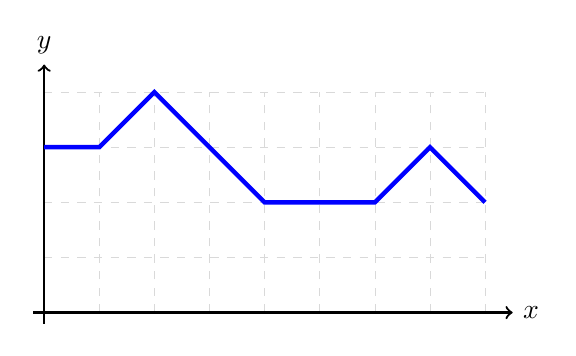
\begin{tikzpicture}[scale=0.7]
			\draw[help lines, color=gray!30, dashed] (0,0) grid (8,4);
			\draw[->,thick] (-0.2,0) -- (8.5,0) node[right] {$x$};
			\draw[->,thick] (0,-0.2) -- (0,4.5) node[above] {$y$};
			\draw[ultra thick,blue] (0,3)--++(1,0)--++(1,1)--++(2,-2)--++(2,0)--++(1,1)--++(1,-1);
		\end{tikzpicture}
	\caption{Example of a lattice path starting at height 3.}
		\label{fig:motzkin}
	\end{center}
\end{figure}

Now, each term in the sum in \eqref{eq:tridiagonal-moments-expansion}
corresponds to a path. Moreover, for each path shape,
there are $O(n)$ summands corresponding to it. The number of
paths of length $k$ starting from a fixed $m$
is finite (independent of $n$ for $m\gg 1$),
so we need to look more closely at the asymptotics of the product
in \eqref{eq:tridiagonal-moments-expansion}. This product
involves chi random variables which depend on $n$, too.

%%%%%%%%%%%%%%%%%%%%%%%%%%%%%%%%%%%%%%%%%%%%%%%%%%%%%%%%%%%%
\subsection{Asymptotics of chi random variables}
\label{sub:chi-asymptotics}
%%%%%%%%%%%%%%%%%%%%%%%%%%%%%%%%%%%%%%%%%%%%%%%%%%%%%%%%%%%%

One additional technical point in analyzing $T/\sqrt{n}$ is to note that $\alpha_j$
is roughly $\sqrt{\beta(n-j)/2}$ for large $n$.
Indeed, we have
\begin{equation*}
	\chi^2_\nu=\sum_{i=1}^\nu Z_i^2,\qquad
	\operatorname{\mathbb{E}}[\chi^2_\nu]=\nu,\qquad
	\operatorname{Var}[\chi^2_\nu]=2\nu.
\end{equation*}
Now, since we are dividing by $\sqrt n$, we have
\begin{equation*}
	\frac{\alpha_j}{\sqrt n}\sim \sqrt{\frac{\beta}{2}}\sqrt{1-\theta},\qquad
	\theta=\frac{j}{n}\in [0,1].
\end{equation*}
This estimate is valid in the ``bulk'' region, that is, when $\theta$ is strictly between $0$ and $1$.

Let us make these estimates more precise.  We have:
\begin{proposition}[Pointwise asymptotics in the bulk]
\label{prop:alpha-bulk}
Fix small $\delta>0$, and let $j$ range so that $\theta_j := j/n \in [\delta,\, 1-\delta]$.
Then for each such $j$, we have\footnote{Here and below, $O_p(\cdot)$ denotes a term that is stochastically bounded at the indicated order as $n\to\infty$. That is, $X_n = O_p(a_n)$ means that for any $\epsilon>0$, there exists $M>0$ such that $\operatorname{\mathbb{P}}(|X_n/a_n| > M) < \epsilon$ for all sufficiently large $n$.}
\[
  \frac{\alpha_j}{\sqrt{n}}
	\;=\; \sqrt{\frac{\beta}{2}\Bigl(1 - \frac{j}{n}\Bigr)}
  \;+\; O_p\Bigl(\frac{1}{\sqrt{n}}\Bigr),
\]
In particular,
\[
  \lim_{n\to\infty} \frac{\alpha_j}{\sqrt{n}}
	\;=\; \sqrt{\frac{\beta}{2}(1-\theta_j)}
  \quad\text{in probability.}
\]
\end{proposition}


\begin{remark}
Outside the bulk region (i.e.\ very close to $j=0$ or $j=n$), one would need a different statement to handle the case $\beta(n-j)$ is not large.
In our application, we only need the bulk behavior.
See also Problem~\ref{prob:edges-in-tridiagonal}.
\end{remark}

Meanwhile, on the diagonal, $d_i/\sqrt{n}$
almost surely vanishes in the limit as $n\to\infty$,
because $d_i$ is standard Gaussian and does not depend on $n$.



%%%%%%%%%%%%%%%%%%%%%%%%%%%%%%%%%%%%%%%%%%%%%%%%%%%%%%%%%%%%
\subsection{Completing the proof: global semicircle behavior}
%%%%%%%%%%%%%%%%%%%%%%%%%%%%%%%%%%%%%%%%%%%%%%%%%%%%%%%%%%%%

Putting the above pieces together, we see that
\begin{equation}
	\label{eq:tridiagonal-moments-discussion}
	\frac{T}{\sqrt n}=
	\frac{1}{n}
	\sum_{i_1,\dots,i_k=1}^n
	\prod_{\ell=1}^k
	\frac{t_{i_\ell i_{\ell+1}}}{\sqrt n},\quad
	i_{k+1}=i_1 \textnormal{ by agreement}.
\end{equation}
The terms in the sum have all $i_{\ell}$'s close together
(there are $k$ indices, and they differ by $\pm1$ from each other).
We
may think that they are close to some $\theta n$, where $\theta\in [0,1]$.
We can consider only the case when $\delta<\theta<1-\delta$ for some fixed small $\delta>0$;
the case of edges does not contribute (see Problem~\ref{prob:edges-in-tridiagonal}).

If at least one of the $t_{ij}$'s in \eqref{eq:tridiagonal-moments-discussion} is
on the diagonal, the term vanishes in the limit. Therefore,
it suffices to consider only the off-diagonal $\alpha_j$'s. The
number of length $k$ walks starting from $m=\theta n$ for $\theta>\delta$ is
just the number of lattice walks with steps $(1,\pm 1)$. This number is $\binom{k}{k/2}$.\footnote{Not Catalan yet!}
(From now on till the end of the section, we assume that
$k$ is even --- the moments become zero for odd $k$).

Fixing the starting location $\theta=\frac{i_\ell}{n}\in(\delta,1-\delta)$, we have
\begin{equation*}
	\prod_{\ell=1}^k
	\frac{t_{i_\ell i_{\ell+1}}}{\sqrt n}\to (\beta/2)^{k/2}(1-\theta)^{k/2}.
\end{equation*}

There is an extra factor $1/n$ in front in \eqref{eq:tridiagonal-moments-discussion},
which is interpreted as transforming the sum over $i_1,\ldots,i_k $
into an integral in $\theta$. We thus see that the moments converge to
\begin{equation*}
	(\beta/2)^{k/2}\binom{k}{k/2}\int_0^1 (1-\theta)^{k/2} \, d\theta=
	(\beta/2)^{k/2}\binom{k}{k/2}\cdot \frac{1}{1+k/2},
\end{equation*}
and we recover our favorite
Catalan moments of the semicircle distribution.

This completes the proof.

\begin{remark}[The factor $(\beta/2)^{k/2}$]
	Note that the factor $\beta^{k/2}$ refers just to the scaling of the Wigner
	semicircle law, and does not affect the semicircle shape. More precisely,
	the limiting semicircle distribution lies from $[-\sqrt{2\beta},\sqrt{2\beta}]$.

	The density of the semicircle distribution on $[-\sqrt{2\beta},\sqrt{2\beta}]$
	is
	\begin{equation*}
		\frac{\sqrt{2-\frac{x^2}{\beta }}}{\pi  \sqrt{\beta }},\qquad |x|<\sqrt{2\beta},
	\end{equation*}
	and the moments are precisely $(\beta/2)^{k/2}C_{k/2}$ (for even $k$).
\end{remark}

\section{Wigner semicircle law via Stieltjes transform}

Let us stay in the tridiagonal setting, and explore a more analytic
method to derive the Wigner semicircle law.

\subsection{Tridiagonal structure and characteristic polynomials}
\label{sec:tridiag-charpoly}

We let
\[
  T - \lambda I =
  \begin{pmatrix}
    d_1 - \lambda & \alpha_1 & 0 & \cdots \\
    \alpha_1 & d_2 - \lambda & \alpha_2 & \ddots \\
    0 & \alpha_2 & d_3 - \lambda & \ddots \\
    \vdots & \ddots & \ddots & \ddots
  \end{pmatrix}.
\]
We want to understand
eigenvalues, that is,
zeros of the characteristic polynomial
$\det(T - \lambda I)$.

\subsubsection{Three-term recurrence for the characteristic polynomial}

As a warm-up, let us consider the characteristic polynomial of a tridiagonal matrix.

For each \(k=1,\dots,n\), denote by \(T_k\) the top-left \(k\times k\) submatrix of \(T\).  Define the \emph{characteristic polynomial} of that block:
\[
  p_k(\lambda) \;=\; \det\bigl(T_k - \lambda I_k\bigr).
\]
By convention, set \(p_0(\lambda)\coloneqq 1\).  Then a determinant expansion argument along the first column gives the following three-term recurrence relation:

\begin{lemma}[Three-Term Recurrence]
\label{lem:3term}
The characteristic polynomial \(p_k(\lambda)\) of the \(k\times k\) tridiagonal matrix \(T_k\) satisfies the three-term recurrence
\[
	p_{k+1}(\lambda)
	\;=\;
	(d_{k+1} - \lambda)\,p_k(\lambda) - \alpha_k^2\,p_{k-1}(\lambda),
	\quad
	k=1,\dots,n-1,
\]µ

\end{lemma}

See also Problem~\ref{prob:Hermite-3-term}.

\subsubsection{Spectral connection and eigenvalues}

The eigenvalues \(\lambda_1,\dots,\lambda_n\) of \(T\) are exactly the roots of \(p_n(\lambda)\).  For any \(\lambda \in \mathbb{C}\), if \(\lambda\) is not an eigenvalue, then \(\bigl(T - \lambda I\bigr)\) is invertible.

When \(\lambda\) is close to a real eigenvalue, the behavior of the resolvent \(\bigl(T-\lambda I\bigr)^{-1}\) becomes large.  Tracking these poles in the complex plane is the key to the resolvent or Stieltjes transform approach.

\subsection{Stieltjes transform / resolvent}
\label{sec:stieltjes-def}

Recall that for a matrix \(A\) with real eigenvalues \(\lambda_1,\dots,\lambda_n\), the \emph{Stieltjes transform} (or Green’s function, or resolvent trace) is
\[
  G_n(z)
  \;=\;
  \frac{1}{n}\,\mathrm{Tr}\bigl[(A - zI)^{-1}\bigr],
  \quad
  z\in \mathbb{C}\setminus\mathbb{R}.
\]
If \(z=x+\mathrm{i}y\) is in the upper half-plane (\(y>0\)), this $G_n(z)$ can be seen as
\[
  G_n(z)
  \;=\;
  \int_{\mathbb{R}}\!\!\frac{d\mu_n(\lambda)}{\lambda - z},
\]
where \(\mu_n = \frac{1}{n}\sum_{k=1}^n \delta_{\lambda_k}\) is the empirical spectral measure.  Equivalently, \(\mathrm{Im}\,G_n(x+\mathrm{i}0^+)\) encodes the density of eigenvalues around \(x\).  Thus, understanding $G_n(z)$ for large $n$ pinpoints the limiting spectral distribution.


Let us apply this to \(A = T/\sqrt{n}\) (an $n\times n$ tridiagonal matrix).  We want
to investigate
\[
	G_n(z)\coloneqq \frac{1}{n}
	\operatorname{Tr}
  \bigl(T/\sqrt{n} - zI\bigr)^{-1},
\]
for complex \(z\).
 Since $T/\sqrt{n}$ has nonzero entries only on the main and first off-diagonals, one can write down a linear recurrence for the entries
$R_{ij}$
of the resolvent
$R(z)=(T/\sqrt{n}-z I)^{-1}$,
from the equation
\[
	\sum_{k}
	\bigl(T/\sqrt{n} - zI\bigr)_{ik}\,R_{kj}
  =
	\mathbf{1}_{i=j}.
\]
We have
\begin{equation*}
	\left(\frac{d_i}{\sqrt{n}}-z\right)R_{ij}
	+
	\frac{\alpha_i}{\sqrt{n}}R_{i+1,j}
	+
	\frac{\alpha_{i-1}}{\sqrt{n}}R_{i-1,j}=
	\mathbf{1}_{i=j}.
\end{equation*}
Let $f_u(\theta)\coloneqq R_{\lfloor n\theta \rfloor ,\lfloor nu \rfloor }$.
Then the above equation becomes
\begin{equation*}
	\left(\frac{d_{\lfloor n\theta \rfloor }}{\sqrt{n}}-z\right)f_u(\theta)
	+
	\frac{\alpha_{\lfloor n\theta \rfloor }}{\sqrt{n}}f_u(\theta+1/n)
	+
	\frac{\alpha_{\lfloor n \theta \rfloor -1}}{\sqrt{n}}f_u(\theta-1/n)=
	\mathbf{1}_{\theta=u}.
\end{equation*}
Scaling with $n$ (and ignoring the boundary conditions and convergence issues), we get
a differential equation for $f_u(\theta)$:
\begin{equation}
	\label{eq:resolvent-diff-eq}
	-z f_u(\theta)+\sqrt{\frac{\beta(1-\theta)}{2}}
	\left[f_u''(\theta)+2f_u(\theta)\right]=\delta(\theta-u).
\end{equation}
The resolvent trace (the Stieltjes transform)
is then the integral of the solution:
\begin{equation*}
	\frac{1}{n}\sum_{i=1}^{n}R_{ii}
	\sim
	G(z)\coloneqq
	\int_0^1 f_\theta(\theta)\,d\theta.
\end{equation*}

\colorbox{green}{\parbox{.7\textwidth}{At this point (2025-01-30), I am stuck on how to pass from
\eqref{eq:resolvent-diff-eq} to the Stieltjes transform $G(z)$.
This would be an excellent topic to explore for a presentation.
See~Problem~\ref{prob:resolvent-diff-eq}.}}

\colorbox{yellow}{\parbox{.7\textwidth}{Update 2025-02-05: Probably,
the limit of $\alpha_j/\sqrt n$ should be taken as $1$ and not as a function of $\tau$.
At least this is what is done in the next approach in \Cref{sub:continued-fractions}.}}


\subsection{Approach via continued fractions}
\label{sub:continued-fractions}

We derive the Wigner semicircle law using the continued
fraction representation of the Stieltjes transform (or
Green's function) associated with a tridiagonal (Jacobi)
matrix. In the Dumitriu--Edelman model for the GUE (let us
assume \(\beta=2\) for simplicity) after appropriate
rescaling, the matrix’s diagonal entries vanish and the
off-diagonal entries become essentially constant in the
bulk. This leads to a homogeneous three-term recurrence for
the corresponding monic orthogonal polynomials. We then show
that the Stieltjes transform of the limiting measure may be
written as an infinite continued fraction, which yields a
quadratic self--consistent equation. Solving that equation
and applying the Stieltjes inversion formula recovers the
semicircle density.

A real symmetric tridiagonal matrix (a \emph{Jacobi matrix}) has the form
\[
J = \begin{pmatrix}
a_0 & b_1 & 0 & \cdots & 0 \\
b_1 & a_1 & b_2 & \ddots & \vdots \\
0 & b_2 & a_2 & \ddots & 0 \\
\vdots & \ddots & \ddots & \ddots & b_{n-1} \\
0 & \cdots & 0 & b_{n-1} & a_{n-1}
\end{pmatrix},
\]
with \(b_j>0\). Associated with \(J\) is a sequence of monic polynomials \(\{p_n(z)\}_{n\ge0}\) defined by the three--term recurrence
\begin{equation}\label{eq:three-term}
\begin{split}
p_0(z)&=1,\\[1mm]
p_1(z)&=z-a_0,\\[1mm]
p_{n+1}(z)&=(z-a_n)p_n(z)-b_n^2\,p_{n-1}(z),\quad n\ge1.
\end{split}
\end{equation}
It is well known that there exists a probability measure \(\mu\) on \(\mathbb{R}\) such that the polynomials \(\{p_n(z)\}\) are orthogonal with respect to \(\mu\).

\medskip

In the Dumitriu--Edelman tridiagonal model for the GUE (with \(\beta=2\)) the matrix is constructed so that, after rescaling by \(\sqrt{n}\), one obtains
\[
\frac{T}{\sqrt{n}} = \begin{pmatrix}
d_1/\sqrt{n} & \alpha_1/\sqrt{n} & 0 & \cdots\\[1mm]
\alpha_1/\sqrt{n} & d_2/\sqrt{n} & \alpha_2/\sqrt{n} & \ddots\\[1mm]
0 & \alpha_2/\sqrt{n} & d_3/\sqrt{n} & \ddots\\[1mm]
\vdots & \ddots & \ddots & \ddots
\end{pmatrix},
\]
with
\[
d_i\sim\mathcal{N}(0,1),\qquad \alpha_j\sim\frac{1}{\sqrt{2}}\chi_{2(n-j)}.
\]
In the large \(n\) limit, the diagonal entries \(d_i/\sqrt{n}\) vanish and (in the bulk) one has
\[
\frac{\alpha_j^2}{n}\to 1.
\]
Thus, in the limit the recurrence coefficients become
\[
a_n=0,\quad b_n=1,
\]
for all \(n\).

\colorbox{yellow}{\parbox{.7\textwidth}{Note 2025-02-05:
This is probably the correct way to approach the global asymptotic behavior of
$T$'s spectrum in connection with the Stieltjes transform.
This should be justified; however, this idea should help to unstick
the argument in \Cref{sec:stieltjes-def}.}}

In this homogeneous case the three-term recurrence \eqref{eq:three-term} reduces to
\[
p_0(z)=1,\quad p_1(z)=z,\quad p_{n+1}(z)=z\,p_n(z)-p_{n-1}(z).
\]

\medskip
The \emph{Stieltjes transform} of the measure \(\mu\) is defined by
\[
m(z)=\int_{\mathbb{R}}\frac{d\mu(x)}{z-x},\qquad z\in\mathbb{C}\setminus\mathbb{R}.
\]
A \textbf{classical result in the theory of orthogonal polynomials}
(e.g., see \cite{sokal2020euler})
is that \(m(z)\) may be written as the continued fraction
\begin{equation}\label{eq:CF}
m(z)=\cfrac{1}{z-a_0-\cfrac{b_1^2}{z-a_1-\cfrac{b_2^2}{z-a_2-\cfrac{b_3^2}{z-a_3-\cdots}}}}.
\end{equation}
In our case, since \(a_n=0\) for all \(n\) and \(b_n=1\) for all \(n\), this simplifies to
\begin{equation}\label{eq:CF_homogeneous}
m(z)=\cfrac{1}{z-\cfrac{1}{z-\cfrac{1}{z-\cfrac{1}{\ddots}}}}.
\end{equation}


Observe that the infinite continued fraction in \eqref{eq:CF_homogeneous} is self--similar; that is, if we denote the entire continued fraction by \(m(z)\), then the tail of the continued fraction is again \(m(z)\). Thus we have the relation
\[
m(z)=\frac{1}{z-m(z)}.
\]
Multiplying both sides by the denominator yields
\[
m(z)\Bigl(z-m(z)\Bigr)=1.
\]
Expanding the left--hand side we obtain the quadratic equation
\begin{equation}\label{eq:quadratic}
m(z)^2-z\,m(z)+1=0.
\end{equation}


The quadratic \eqref{eq:quadratic} has the solutions
\[
m(z)=\frac{z\pm\sqrt{z^2-4}}{2}.
\]
To determine the correct branch, recall that for \(z\) in the upper half--plane (\(\operatorname{Im}(z)>0\)) we must have \(\operatorname{Im}\,m(z)>0\). The proper solution is
\begin{equation}\label{eq:m_solution}
m(z)=\frac{z-\sqrt{z^2-4}}{2},
\end{equation}
where the square root is defined so that \(\sqrt{z^2-4}\sim z\) as \(z\to\infty\) and \(\operatorname{Im}\sqrt{z^2-4}>0\) when \(\operatorname{Im}(z)>0\).


The density \(\rho(x)\) of the measure \(\mu\) is recovered from the Stieltjes transform via the inversion formula:
\[
\rho(x)=\frac{1}{\pi}\lim_{\epsilon\to0^+}\operatorname{Im}\,m(x+i\epsilon).
\]
For \(x\) in the interval \((-2,2)\) one computes that
\[
\sqrt{(x+i\epsilon)^2-4}\;\xrightarrow[\epsilon\to0^+]{}\; i\sqrt{4-x^2}.
\]
Thus, from \eqref{eq:m_solution} we have, for \(x\in(-2,2)\),
\[
m(x+i0)=\frac{x-\mathrm{i}\sqrt{4-x^2}}{2}.
\]
Taking the imaginary part gives
\[
\operatorname{Im}\,m(x+i0)=\frac{\sqrt{4-x^2}}{2},
\]
so that
\[
\rho(x)=\frac{1}{\pi}\operatorname{Im}\,m(x+i0)=\frac{1}{2\pi}\sqrt{4-x^2},\quad x\in(-2,2).
\]
This is precisely the celebrated Wigner semicircle law.



\section{Determinantal point processes (discrete)}
\label{sec:determinantal}

We are now going to start the discussion of the local eigenvalue
behavior at $\beta=2$, started in \Cref{subsec:beta2-case}.
We begin with a general discussion of \emph{determinantal point processes} (DPPs),
starting in discrete world. The continuous world is going to be considered in the next
\href{https://lpetrov.cc/rmt25/rmt25-notes/rmt2025-l05.pdf}{Lecture 5}.

In this section, we introduce \emph{determinantal point processes (DPPs)}
over a discrete state space and explore some of their properties.
Our main reference is \cite{Borodin2009}.

\medskip

\noindent\textbf{Setup.} Let \(\mathfrak{X}\) be a (finite or countably infinite)
discrete set endowed with the counting measure \(\mu\).
A \emph{point configuration} on \(\mathfrak{X}\) is any subset \(X\subset \mathfrak{X}\),
finite or infinite, with no repeated points.\footnote{Some texts allow
multiplicities, but we disallow them here.}
We write \(Conf(\mathfrak{X})\) for the set of all point configurations,
which carries the natural \(\sigma\)-algebra generated by the functions
\(\mathbf{1}_{\{x\in X\}}\), \(x\in\mathfrak{X}\). A \emph{random point process} \(P\)
on \(\mathfrak{X}\) is a probability measure on \(Conf(\mathfrak{X})\).

\begin{definition}[Determinantal point process]
\label{def:dpp-discrete}
A random point process \(P\) on a discrete set \(\mathfrak{X}\) is \emph{determinantal}
if there exists a kernel function \(K:\mathfrak{X}\times\mathfrak{X} \to \mathbb{C}\) such that
for every finite collection of pairwise distinct points \(x_1,\dots,x_n\in \mathfrak{X}\),
\begin{equation}
\label{eq:DPP-def}
\operatorname{\mathbb{P}}\{x_1,\dots,x_n\in X\} = \det\bigl[K(x_i,x_j)\bigr]_{i,j=1}^n.
\end{equation}
That is, all finite-dimensional distributions of \(P\) take a determinantal form.
The function \(K\) is called a \emph{correlation kernel} for \(P\).
\end{definition}

\noindent\textbf{Correlation functions and the kernel.}
The condition \eqref{eq:DPP-def} captures all finite-dimensional distributions of \(P\).
Equivalently, let
\[
	\rho_n(x_1,\dots,x_n) \coloneqq \operatorname{\mathbb{P}}\{\text{there is a particle at each }x_i\}
\]
for distinct \(x_1,\dots,x_n\). In the discrete setting, \(\rho_n\) is
sometimes called the \emph{(unordered) correlation function}. The process is
determinantal if and only if
\[
\rho_n(x_1,\dots,x_n) = \det\bigl[K(x_i,x_j)\bigr]_{i,j=1}^n
\quad
\text{for each }n\ge1.
\]

\noindent\textbf{Basic properties.} If \(P\) is a DPP with correlation kernel
\(K\colon \mathfrak{X}\times\mathfrak{X}\to\mathbb{C}\), then for any subset \(I\subset \mathfrak{X}\),
\begin{equation}
\label{eq:prob-empty-set-DPP}
\operatorname{\mathbb{P}}\{X\cap I = \varnothing\} = \det\bigl[\mathbf{1} - K_I\bigr],
\end{equation}
where \(K_I\) is the operator \(\bigl[K(x,y)\bigr]_{x,y\in I}\)
(viewed as a matrix if \(\mathfrak{X}\) is finite, or an infinite matrix if \(\mathfrak{X}\) is
countably infinite with convergent sums). More generally, if \(I_1,\dots,I_m\subset \mathfrak{X}\)
are disjoint subsets, then the joint event \(\{|X\cap I_k|=n_k\text{ for }1\le k\le m\}\)
can be expressed via the determinant
\(\det\bigl[\mathbf{1}-\sum_{k=1}^m z_k K_{I_k}\bigr]\)
and its derivatives.

\begin{remark}
For any function \(\phi:\mathfrak{X}\to\mathbb{C}\) such that the operator
\(\bigl[(1-\phi(x))K(x,y)\bigr]_{x,y\in\mathfrak{X}}\) is trace class, the
exponential generating function for \(\phi\) is
\[
\mathbb{E}\Bigl[\prod_{x\in X}\phi(x)\Bigr] = \det\bigl[\mathbf{1} - (1-\phi)K\bigr].
\]
This identity makes determinantal point processes more tractable than general processes.
\end{remark}

\subsubsection*{A key example: one-dependent processes on \texorpdfstring{$\mathbb{Z}$}{}}
We highlight an important application from \cite{borodin2010adding} that connects
\emph{1-dependent} processes on an integer segment (or a finite subset of \(\mathbb{Z}\))
to determinantal processes. A point process \(P\) on \(\mathbb{Z}\) is \emph{1-dependent} if,
for any two disjoint finite sets \(A,B\subset\mathbb{Z}\) with \(\mathrm{dist}(A,B)\ge2\),
the correlation function factorizes:
\[
\rho_{|A|+|B|}(A\cup B) = \rho_{|A|}(A)\,\rho_{|B|}(B).
\]


\begin{theorem}[{\cite[Thm.~1.1]{borodin2010adding}]}]
\label{thm:1-dependent-implies-dpp}
Any one-dependent point process on a finite segment of \(\mathbb{Z}\) is a determinantal process.
Moreover, its correlation kernel \(K\) can be explicitly computed.
\end{theorem}

\begin{example}[Adding a list of numbers]
\label{ex:adding-numbers}
Consider an i.i.d.\ sequence of random variables \(\{\xi_j\}\) (each taking values in \(\{0,1\}\)),
and define the partial sums \(S_n = \sum_{j=1}^n \xi_j\). The occupancy process,
marking site \(S_n\) as “occupied,” forms a 1-dependent sequence. By \Cref{thm:1-dependent-implies-dpp},
it is thus determinantal.
\end{example}

\section{Application of determinantal processes to random matrices at \texorpdfstring{$\beta=2$}{beta=2}}

In this final section of the lecture, we illustrate how the theory of determinantal point processes (DPPs)
introduced in \Cref{sec:determinantal}
applies to the study of local eigenvalue statistics of random matrices.
We concentrate on the \(\beta=2\) setting, where DPPs typically
govern the joint behavior of eigenvalues at microscopic (local)
scales in the \emph{bulk} and at the \emph{edge} of the spectrum.
We also include a simpler example of a Poisson process to highlight
the role of correlation functions.

\subsection{Local eigenvalue statistics (bulk and edge scaling limits)}
\label{subsec:local-stats-intro}

Given an \(n\times n\) random Hermitian matrix \(W\) whose eigenvalues
\(\lambda_1 \ge \lambda_2 \ge \cdots \ge \lambda_n\) are real,
we often want to study the \emph{local arrangement} of the eigenvalues:
\begin{itemize}
	\item \emph{Bulk regime:}
		eigenvalues near some interior point \(\alpha\)
		of the limiting (global) spectral support, rescaled so that we see
		``microscopic'' spacing on the order of \(O(\tfrac1n)\).
		For Wigner or Gaussian ensembles, one typically looks at a point
		\(\alpha\) in the interior \((-2,2)\) of the semicircle support
		and then rescales eigenvalues around \(\alpha\) by the typical local spacing \(1/(n\rho(\alpha))\). Here $\rho(\alpha)$ is the density of eigenvalues at \(\alpha\),
		which is semicircle density in the Wigner case.
	\item \emph{Edge regime:}
		eigenvalues near an endpoint of the support
		(for instance, near \(x=2\) for the semicircle distribution).
		One then uses a rescaling of order \(n^{2/3}\) (in many classical models)
		to see nontrivial statistics describing how eigenvalues ``peel off'' near the boundary.
\end{itemize}

In both cases, one replaces the original sequence of eigenvalues \(\{\lambda_i\}\) by
a \emph{point process} on \(\mathbb{R}\).  The \emph{bulk scaling} leads to the sine-kernel process (e.g.\ \(\sin(\pi(x-y))/(\pi(x-y))\) in the GUE) or more generally to other determinantal processes.
The \emph{edge scaling} typically leads to the Airy-kernel process.
For Gaussian ensembles at \(\beta=2\), these processes are determinantal, and one can explicitly
write correlation kernels involving special functions (sine, Airy, and more generally Hermite polynomials).

\subsection{Correlation functions and densities}
\label{subsec:correlation-functions}

We recall from \Cref{sec:determinantal} (in the discrete setting) that a point process \(\mathcal{X}\) on a space \(\mathfrak{X}\) can be described by its \emph{correlation functions} \(\{\rho_k\}_{k=1}^\infty\). In the continuous setting (e.g.\ \(\mathfrak{X}=\mathbb{R}\) or an interval), these are defined so that
\begin{equation}
  \rho_k(x_1,\dots,x_k)\,dx_1\cdots dx_k
  \;=\;
  \text{(probability that there is a particle in each small set $dx_i$ near $x_i$, for $1\le i\le k$)}.
\end{equation}
Equivalently, \(\rho_k\) is the \(k\)-th \emph{(unordered) joint density} of the process.  In particular,
\[
  \rho_1(x)\,dx
  \;=\;
  \text{expected number of particles in a small interval of length $dx$ near $x$.}
\]
For a \emph{determinantal} point process in the continuous setting, there is a kernel \(K(x,y)\) such that
\begin{equation}
  \label{eq:rho-k-dpp-cont}
  \rho_k(x_1,\dots,x_k)
  \;=\;
  \det\bigl[K(x_i,x_j)\bigr]_{i,j=1}^k
  \quad
  \text{for each $k\ge1$}.
\end{equation}
The simplest example is the \emph{Poisson process} (see \Cref{subsec:poisson-example}), which in fact is \emph{not} determinantal but helps illustrate how correlation functions characterize clustering or repulsion of points.

\subsection{Poisson process example}
\label{subsec:poisson-example}

A \emph{Poisson point process with intensity} \(\lambda>0\) on \(\mathbb{R}\) is defined by:
\begin{itemize}
	\item Particles are scattered independently over real line,
	\item The expected number of particles in an interval \(I\subset \mathbb{R}\) is \(\lambda|I|\).
\end{itemize}
Equivalently, one often states that the number of points in any interval \(I\) follows a Poisson(\(\lambda|I|\)) distribution, and disjoint intervals are filled independently.  One can also check that the correlation functions factorize completely:
\[
\rho_k(x_1,\dots,x_k) \;=\; \lambda^k.
\]
Hence, in the Poisson process, there is no ``interaction'' or ``repulsion'' between points: the position of one particle does not affect the probability of having other particles nearby.  In contrast, a determinantal point process typically exhibits \emph{repulsion}: if you know a particle is present near \(x\), it lowers the density of particles nearby.  This effect is crucial in random matrix ensembles at \(\beta=2\).




\appendix
\setcounter{section}{3}

\section{Problems (due 2025-02-28)}

\subsection{Eigenvalue density of G$\beta$E}

Read and understand the main principles of the
proof of \Cref{thm:DE-joint-eigenvalue-density}
in \cite{dumitriu2002matrix}.

\subsection{Chi-square mean and variance}

Let $X$ be a random variable with $\chi^2_\nu$ distribution. Compute the mean and variance of $X$.
(If $\nu$ is an integer, you can use the fact that $\chi^2_\nu$ is a sum of $\nu$ independent squares of standard normal random variables.
How to extend this to non-integer \(\nu\)?)

\subsection{Edge contributions in the tridiagonal moment computation}
\label{prob:edges-in-tridiagonal}

Show that the cases when the $i_{\ell}$'s are close to the edge ($\theta=0$ or $1$)
in \eqref{eq:tridiagonal-moments-discussion}
do not contribute to the limit of the moments.

\subsection{Hermite polynomials and three-term recurrence}
\label{prob:Hermite-3-term}

Show that the monic Hermite polynomials $H_k(x)$
\eqref{eq:hermite-polynomial}
satisfy the three-term recurrence relation
\begin{equation*}
	\label{eq:hermite-3-term}
	H_k(x) = x H_{k-1}(x) - (k-1) H_{k-2}(x).
\end{equation*}

\subsection{}
\label{prob:Vandermonde-determinant}

Compute the determinant
\begin{equation*}
	\det\left[
		\begin{array}{cccc}
			1 & 1 & \cdots & 1 \\
			x_1 & x_2 & \cdots & x_n \\
			x_1^2 & x_2^2 & \cdots & x_n^2 \\
			\vdots & \vdots & \ddots & \vdots \\
			x_1^{n-1} & x_2^{n-1} & \cdots & x_n^{n-1}
		\end{array}
	\right].
\end{equation*}

\subsection{Gap probabilities}

\begin{enumerate}
	\item
Prove identity
\eqref{eq:prob-empty-set-DPP} for DPPs.
\item Prove the generalization computing
	\(\{|X\cap I_k|=n_k\text{ for }1\le k\le m\}\).
\end{enumerate}


\subsection{Stieltjes transform approach for tridiagonal matrices}
\label{prob:resolvent-diff-eq}

Complete the derivation from \Cref{sec:stieltjes-def} to obtain the limiting Stieltjes transform $G(z)$ for the tridiagonal matrix $T/\sqrt{n}$.

\begin{remark}
	This is more of a literature search. It is extensive, and
	would make an excellent topic for a presentation.
\end{remark}

\bibliographystyle{alpha}
\bibliography{bib}


\medskip

\textsc{L. Petrov, University of Virginia, Department of Mathematics, 141 Cabell Drive, Kerchof Hall, P.O. Box 400137, Charlottesville, VA 22904, USA}

E-mail: \texttt{lenia.petrov@gmail.com}


\end{document}
